
\documentclass[a4paper,12pt]{article}

\usepackage{graphicx} % Required for inserting images
\usepackage{amsmath,amssymb,amsfonts}
\usepackage{subcaption}
% -----------------------
% Package Imports
% -----------------------

% Set page margins
\usepackage[a4paper, top=1in, bottom=0.8in, left=1.1in, right=0.8in]{geometry}

% Use Times New Roman font
\usepackage{times}

% Add page numbering
\pagestyle{plain}

% Enable graphics inclusion
\usepackage{graphicx}
\usepackage{float}
% Enable code listings
\usepackage{listings}
\usepackage{xcolor} % For customizing code colors
\setlength{\parindent}{0pt}
\usepackage{multirow}

\setlength{\parindent}{0pt}
\usepackage{sectsty}
\sectionfont{\fontsize{12}{15}\selectfont}


\begin{document}
	\section{Experiment No. 5}
	
	\section{Experiment Title }
Synchronization of an alternator with an infinite bus using lamp method.
	
	\section{Objective}
	
	The objectives of this lab are as follows:
	\begin{itemize}
		\item 	To use the three-lamp approach to synchronize a three-phase alternator with an infinite bus.
		\item 	To observe the power sharing by varying the field current and field resistance.
	
		
		
	\end{itemize}
	
\section{Theory}

To synchronize an alternator with an infinite bus, the \textbf{phase sequence}, \textbf{voltage}, and \textbf{frequency} of the alternator must match those of the infinite bus. An \textbf{infinite bus} is defined as a power source whose voltage and frequency remain constant regardless of load variations.

Traditionally, synchronization was performed using the \textbf{three-lamp method}, and the synchronizing switch was closed when the lamps indicated the proper conditions visually.

The conditions for synchronizing a generator with an infinite bus are as follows:

\begin{enumerate}
	\item The terminal voltage of the generator must be equal to the voltage of the infinite bus.
	\item The phase sequence of the generator must match that of the infinite bus.
	\item The phase angle between the corresponding phases must be zero.
	\item The frequency of the generator should be slightly greater than that of the infinite bus during synchronization.
\end{enumerate}
	\begin{figure}[H]
	\centering
	\centering
	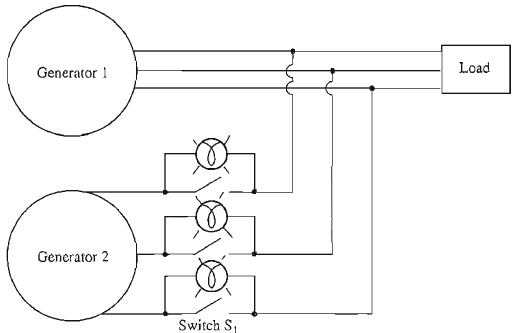
\includegraphics[width=0.65\textwidth]{Images/1}
	\caption{The three-light-bulb method for
		checking phase sequence.}
	
	
	
	
	
\end{figure}
When a generator operates in isolation, its terminal voltage depends on the load, while the generated voltage is determined by the field current, and its frequency is governed by the rotational speed of the alternator.

If \( n \) is the speed of the rotor in revolutions per minute (rpm), and \( P \) is the number of poles in the armature, then the frequency \( f \) of the generated voltage is given by:

\[
f = \frac{nP}{120}
\]

The generated voltage \( E_a \) can be expressed as:

\[
E_a = k \phi \omega
\]

where:
\begin{enumerate}
	\item \( k \) is a machine constant,
	\item \( \phi \) is the magnetic flux per pole,
	\item \( \omega \) is the angular speed of the rotor (in rad/s).
\end{enumerate}

Once the generator is synchronized and connected to the infinite bus, its frequency becomes locked to that of the grid and does not change with variations in field excitation. In this condition:

\begin{enumerate}
	\item \textbf{Active power} delivery is controlled by changing the \textbf{prime mover input} (i.e., mechanical power).
	\item \textbf{Reactive power} delivery is controlled by changing the \textbf{field current}.
\end{enumerate}

However, the \textbf{terminal voltage} remains fixed by the infinite bus and does not vary with the field current.

	\section{Circuit Diagram}
	\begin{figure}[H]
		\centering
			\centering
			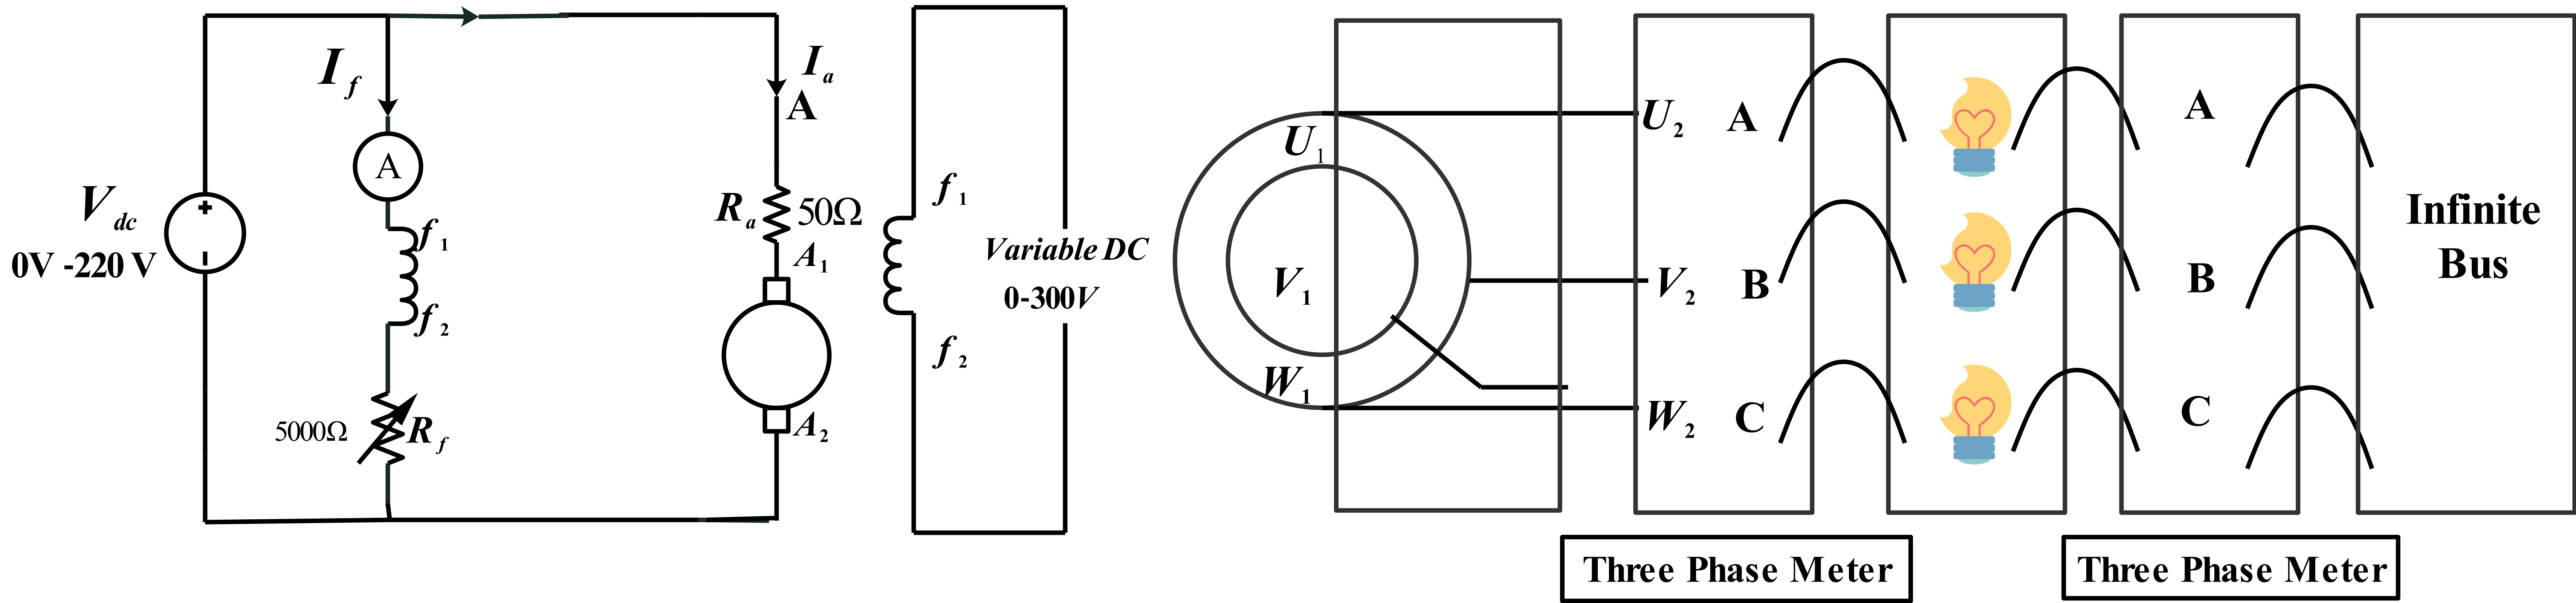
\includegraphics[width=1\textwidth]{Images/exp05}
			\caption{Circuit Diagram of Synchronization of an alternator with an infinite bus using lamp method.}
			
	
		
		
		
	\end{figure}
	\newpage
	\section{Required Apparatus}
	\begin{enumerate}
		\item \textbf{DC Motor}
		\begin{enumerate}
			\item Power: 300W , Speed: 3000 rpm
			\item Voltage: 220V
			\item \textbf{Excitation (Series)}: D1-D2, Current: 1.9A, \textbf{Excitation (Separate)}: F1-F2, Current: 1.8A, Excitation Voltage: 220V, Excitation Current: 0.1A
			
		\end{enumerate}
		
		\item \textbf{Synchronous Generator}
		\begin{enumerate}
			\item Power: 350W ,Power Factor: $\cos\phi = 1$ ,Speed: 3000 rpm
			
			\item Voltage: 400V (star) / 230V (delta) ,Current: 0.7A (star) / 1.2A (delta) 
			\item Excitation Voltage: 220V ,Excitation Current: 0.45A
			
		\end{enumerate}
		
		\item \textbf{Resistors}
		\begin{enumerate}
			\item 50$\Omega$: Power = 500W, Current = 3.16A
			\item 200$\Omega$: Power = 500W, Current = 1.58A
			\item 5000$\Omega$: Power = 500W, Current = 0.31A
		\end{enumerate}
		
		\item \textbf{Tachometer}
		\begin{enumerate}
			\item For 0.6V/rev: 300V at 5000 RPM , For 2mV/rev: 10V at 5000 RPM
			\item Maximum Current: 0.07A
			\item Maximum Speed: 5000 RPM
		\end{enumerate}
		
		\item \textbf{AC Multimeter}
		\begin{enumerate}
			\item 500V AC RMS
			\item 5A
		\end{enumerate}
	\end{enumerate}
	\newpage
	\section{Data Table}
	
		\begin{table}[H]
		\centering
			\caption{: Table for Field Current vs Active \& Reactive Power}
		
			\begin{tabular}{|c|c|c|}
			\hline
			\textbf{\begin{tabular}[c]{@{}c@{}}Field   Current (If)    \\ (Amp)\end{tabular}} & \textbf{\begin{tabular}[c]{@{}c@{}}Active   Power (P)   \\ (Watt)\end{tabular}} & \textbf{\begin{tabular}[c]{@{}c@{}}Reactive   Power (Q)    \\ (VAR)\end{tabular}} \\ \hline
			0.235                                                                              & 2.7                                                                                & -2.3                                                                                \\ \hline
			0.261                                                                               & 5.3                                                                                & -3.2                                                                                \\ \hline
			0.275                                                                               & 3.4                                                                                & -3.5                                                                                \\ \hline
			0.282                                                                               & 4.5                                                                                & -3.4                                                                                \\ \hline
			0.297                                                                               & 1.6                                                                                & -2.1                                                                                \\ \hline
		\end{tabular}
		
		
\end{table}
	\begin{table}[H]
		\centering
	
		\caption{Table for Speed vs Active \& Reactive Power } 
			
		
			\begin{tabular}{|c|c|c|}
			\hline
			\textbf{\begin{tabular}[c]{@{}c@{}}Speed(ns)   \\ (RPM)\end{tabular}} & \textbf{\begin{tabular}[c]{@{}c@{}}Active Power (P)   \\ (Watt)\end{tabular}} & \textbf{\begin{tabular}[c]{@{}c@{}}Reactive Power (Q)    \\ (VAR)\end{tabular}} \\ \hline
			\multirow{5}{*}{3040}                                                    & 2.4                                                                              & -3.8                                                                              \\ \cline{2-3} 
			& 0.3                                                                              & -2.4                                                                              \\ \cline{2-3} 
			& 3.4                                                                              & -3.7                                                                              \\ \cline{2-3} 
			& 5.3                                                                              & -3.6                                                                              \\ \cline{2-3} 
			& 5.5                                                                              & -3.7                                                                              \\ \hline
		\end{tabular}
		
		% Sub-table (b) caption
		
	\end{table}
	
	\section{Discussion}
	In this experiment, a three-phase alternator was synchronized with an infinite bus using the three-lamp method. Proper synchronization was confirmed when all three lamps were observed to dim simultaneously, indicating that voltage, frequency, and phase sequence were matched. Initially, issues related to phase sequence were resolved by interchanging two of the phase wires.
	
	It was observed that an increase in the generator speed resulted in an increase in active power, while the reactive power remained negative. When the field current was varied at a constant speed, significant changes were noted primarily in reactive power. These observations confirmed that active power was controlled by the rotor speed, whereas reactive power was controlled by the excitation level.
	
	
\end{document}
